\NeedsTeXFormat{LaTeX2e}
\documentclass[11pt]{article}
\usepackage[utf8]{inputenc}
\usepackage[T1]{fontenc}
\usepackage{ae}
\usepackage[intlimits, sumlimits, namelimits]{amsmath}
\usepackage{bbm}
\newcommand{\inp}[1]{\ensuremath{\left(#1\right)}}
\newcommand{\sqr}{\ensuremath{^{2}}}
\newcommand{\cube}{\ensuremath{^{3}}}
\newcommand{\set}[1]{\ensuremath{\mathbbm{#1}}}
\newcommand{\norm}[1]{\ensuremath{\left|#1\right|}}
\newcommand{\svec}[3]{\ensuremath{\inp{\hspace{-.8ex}\begin{array}{r}#1\\#2\\#3\end{array}\hspace{-.4ex}}}}
\newcommand{\entspr}{\ensuremath{\,\,\hat{=}\,\,}}%
\newcommand{\dx}[1][x]{\ensuremath{\textnormal d #1}}

% For stupid thinkos:
\newcommand{\cross}{\times}

\usepackage{array}
\setlength{\extrarowheight}{.2mm}
\usepackage{hyperref}
\usepackage{graphics,graphicx,fancyvrb}
%Raender einstellen
%\usepackage[a4paper, margin=15mm, top=30mm]{geometry}
\usepackage[a4paper]{geometry}
\usepackage{lastpage}
\usepackage{fancyhdr}
	\lhead{Moritz Lenz}
	\chead{\bfseries{-- \thepage\ --}}
	\rhead{\thetitle}
	\lfoot{}
	\rfoot{}
	\cfoot{}
	\pagestyle{fancy}
\pagestyle{empty}

\sffamily

%Kopfzeile

\author{Moritz Lenz}
\title{Theory}
\begin{document}
\maketitle

Consider a two-dimensional conductor of width $W$ and length $L$. If these two
dimensions  are large enough, the conductance is

\begin{align}
    G = \sigma \frac{W}{L}
\end{align}

where $\sigma$ is a material specific parameter, and independent of the
geometry of the conductor. \emph{Large enough} means in this context
specifically that both lengths are large compared to all of three
characteristic lengths: the Fermi wavelength, the mean free path and the
phase-relaxation length.

The mean free path is the average distance which a charge carrier can travel
before it is scattered (by an impurity, electrons or phonons), and thus loses
momentum.

If the length of the conductor is smaller than the mean free path, most
electrons travel through it without scattering, and one could naively assume
that this means the resistance is zero.

Still experiments show that a finite resistance can be observed. That's
because the sample can't be measured in isolation; it is attached to the
macroscopic measuring system through \emph{leads}. Even if the leads are very
good conductors themselves, a contact resistance arises. So the theory has to
take into account both the sample and the leads.

\subsection*{Landauer Formula}

\begin{figure}
    \begin{center}
        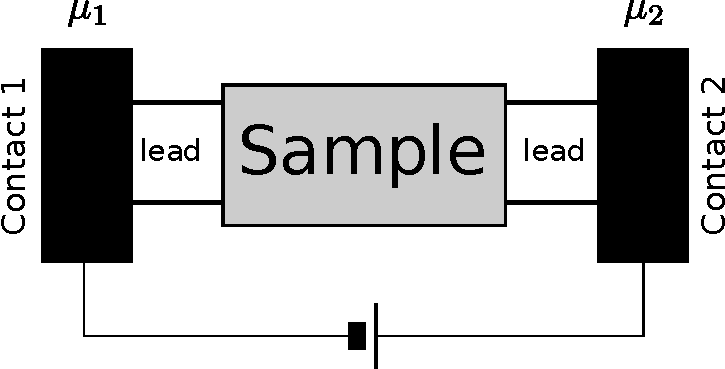
\includegraphics[width=0.5\textwidth]{sample-leads}
    \end{center}
    \caption{Schematic setup to derive the Landauer Formula}
    \label{fig:sample-leads}
\end{figure}

The sample is attached to two leads, which we assume to be perfect, ballistic
conductors with $M$ modes each. We assume that the contacts are
reflectionless, that is electrons can travel from the sample into the contacts
without reflection.

This means that the $k_x$ states in the left lead are occupied by electrons
coming from contact 1, and thus have the same electrochemical potential as
the contact, $\mu_1$. Likewise the $-k_x$ states in the right lead have the
potential $\mu_2$.

At zero temperature, only electrons with energies between $\mu_1$ and $\mu_2$
are transported, and the influx from the left lead is
$I_1^+ = (2e/h)M(\mu_1-\mu_2)$. We call the transmission probability through
the sample $T$, so the outflux from lead 2 is $I_2^+ = T I_1^+$, the rest
is reflected back: $I_1^- = (1-T) I_1^+$. The net current $I$ then is

\begin{align*}
    I = I_1^+ - I_1^- = \frac{2e}{h} M T (\mu_1 - \mu_2)
\end{align*}

The conductance is

\begin{align*}
    G = \frac{I |e|}{\mu_1 - \mu_2} = \frac{2 e^2}{h} MT
\end{align*}

\end{document}

% vim: ts=4 sw=4 expandtab spell spelllang=en_us tw=78
